\chapter{Introduction}

\devnote{This chapter is currently being written\ldots}

%FIXME: Automation of CMM, FEniCS, purpose of DOLFIN,
%FIXME: PSE for differential equations, C++ interface of FEniCS, etc

%------------------------------------------------------------------------------
\section{The FEniCS project}
\index{FEniCS}
\index{automation}

% FIXME: Automation of CMM, other components of \fenics{}

%------------------------------------------------------------------------------
\section{The finite element method}
\index{finite element method}

% FIXME: Automation of discretization

%------------------------------------------------------------------------------
\section{Overview}

\dolfin{} is implemented as a C++ library and can be used either as a
stand-alone solver, or as a tool for the development and
implementation of new methods. To simplify usage and emphasize
structure, \dolfin{} is organized into three levels of abstraction,
referred to as \emph{kernel level}, \emph{module level}, and
\emph{user level}, as shown in Figure \ref{fig:components}.  Core
features, such as the automatic evaluation of variational forms and
adaptive mesh refinement, are implemented as basic tools at kernel
level. At module level, new solvers/modules can be assembled from
these basic tools and integrated into the system. At user level, a
model of the form is specified and solved, either using one of the
built-in solvers/modules or by direct usage of the basic tools.

\begin{figure}[htbp]
  \begin{center}
    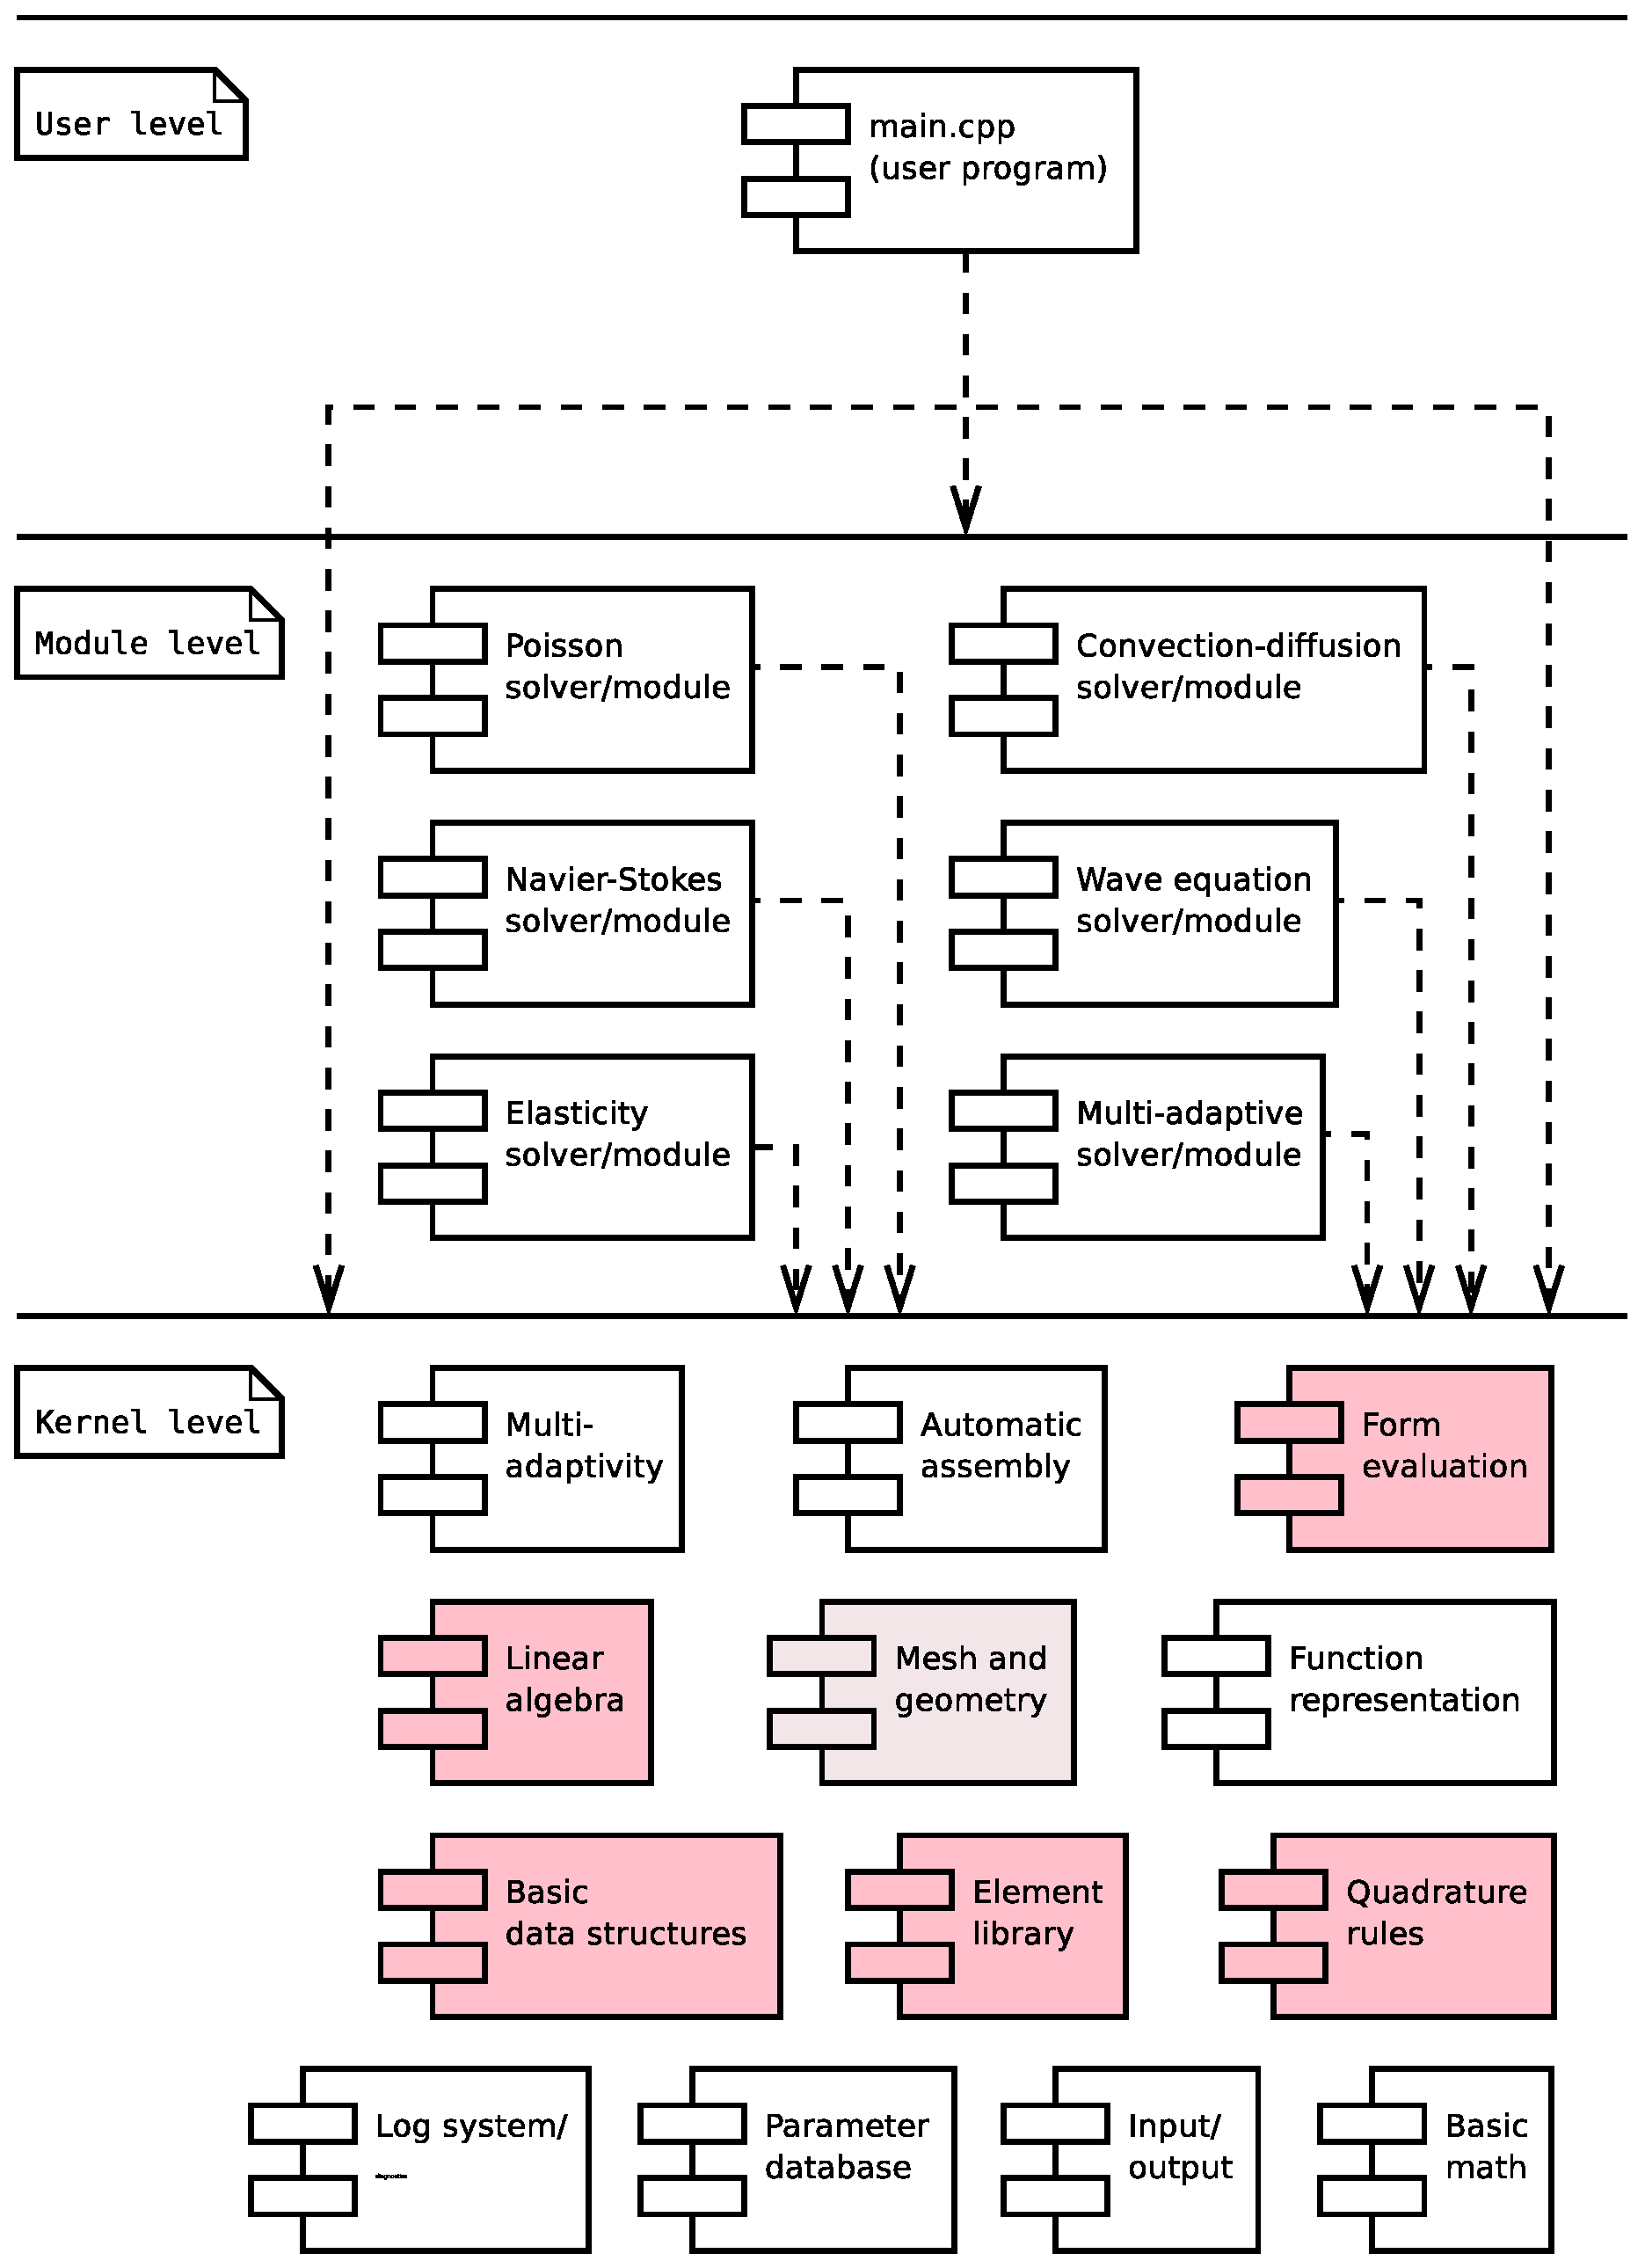
\includegraphics[width=12.5cm]{eps/dolfin-components.eps}
    \caption{Simplified component diagram of \dolfin{}.}
    \label{fig:components}
  \end{center}
\end{figure}
